\chapter{Introduction} \label{ch:introduction}
In recent years, the interest in unmanned aircraft vehicles (UAVs) research has increased substantially. This is due to the several potential new services this type of robotic devices offers, such as search and rescue, observation, mapping, inspection, etc. On the other hand, smartphones have become essential devices for humans and easily acquirable development tools. The interaction between these two technologies allows the development of low cost aerial robots based on an everyday item such as smartphones, facilitating both the distribution of its control software and its implementation by other researchers.
\\\\
\section{Motivation}
Quadrotor control is both a difficult and interesting problem. As established by \cite{Liu2015} and \cite{Lopez2015}, quadrotor dynamics are affected by nonlinearity, parameters perturbations, uncertainties and disturbances: these include unknown and variable payloads, aerodynamical parameters of the system, wind changes, and sensors inaccuracies. Several studies have been developed in designing optimal and robust controllers that allow UAVs to fly and accomplish missions rejecting disturbances and being robust to parameter uncertainties as seen in \cite{Jung2014, Kohno2014, Shang2016, Salazar2014}.\\\\
Although there are embedded systems with high computational capacity that can serve as controllers of a quadrotor, smartphones are available, easily accessible for people and also have a large computational capacity, hence multiple instrumentation and communication elements integrated in the same device. In the last years, computing capacity and sensor technology in smartphones have decreased in price but increased in performance. Smartphones have become an inexpensive tool capable of commanding an UAV. The challenge then, is to use smartphones as quadrotor flight controllers for autonomous flights following specific missions, considering that the phones today are powerful computers that include elements for sensing, processing and communication.
\\\\
This research project aims to design and implement algorithms that will be executed in a smartphone to estimate and control the dynamics of a quadrotor. This project confronts several challenges such as using a smartphone as a hardware development platform, trying to use a non real-time operating system for real-time applications, designing optimal and high order controllers using Java, and executing that controllers in a smartphone. 
\\\\
\section{Unmanned Aircraft Vehicles (UAV)}
An UAV is an aircraft capable of flying without having a human on board. This aircrafts are commonly known as `drones' due to the similarity of the sound they emit with that of a male bee (drone). Although they can perform flight missions in a completely autonomous way, the UAVs are complemented with remote display and control systems (Ground Control Station - GCS), and communication systems between the UAV and the GCS. These three components describe what is known as Unmanned Aircraft Systems (UAS).\\\\
The UAS were initially designed for military applications, where the presence of a human could be at high risk \cite{Bouabdallah2007}. However, their use has been widely extended to multiple applications such as education \cite{Rahman2017}, agriculture \cite{Garcia2015}, search and rescue \cite{KumarS2015}, delivery \cite{Gatteschi2015}, research \cite{Gonzalez2012}, among others. 
\\\\
UAVs are modelled as rigid bodies with freedom of movement in a three-dimensional space, hence have six degrees of freedom ($DoF$), three translational (position) and three rotational (attitude). These aircrafts are classified mainly according to the propulsion direction exerted by the actuators. Thus, there are two groups of UAVs: Fixed-wing and Rotary-wing UAVs, which are described below.

\subsection{Fixed-Wing UAVs}
A fixed-wing UAV is an aircraft which consists of an airframe attached to a rigid wing that generates lift using the UAVs forward airspeed and geometry. This type of UAVs need a constant forward movement in order to produce air flow around its wing, which can be generated by the thrust of propeller pushing the air flow in opposite direction of the UAV movement, or flying against to the wind. An example of a fixed-wing UAV is shown in Fig. \ref{fig:fixedwing}.
\begin{figure}[h]
\begin{center}
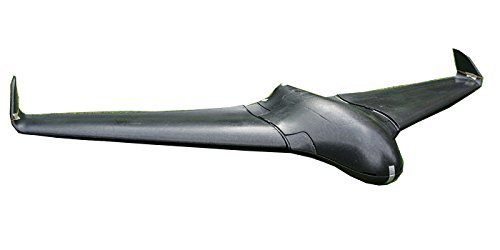
\includegraphics[width=9.6cm]{fixedwinguav.jpg}    
\caption[Skywalker X8 fixed-wing UAV]{Skywalker X8 fixed-wing UAV\protect\footnotemark} 
\label{fig:fixedwing}
\end{center}
\end{figure}
\footnotetext{Fixed-wing UAV image taken from \url{https://goo.gl/LNEriU}}
\\\\Since they need a minimum airspeed to achieve their lift in flight, these aircrafts require a runway or catapult for taking off and landing. However, its geometry allows to achieve long-term flights (greater than $60$ minutes) at high speeds (greater than $20\ m/s$) by taking advantage of its aerodynamic efficiency. Also, they are capable of carrying big and heavy payloads without significantly affecting the duration of the flight.
\\\\
The six $DoF$ of a fixed-wing UAV are controlled using elevators, ailerons and rudders, which are control surfaces built in the wing. The use of the control surfaces allows rotations to be made about any of the three perpendicular axes that intersect at the UAV center of gravity ($CoG$), and therefore control the rotational $DoF$. The translational $DoF$ are directly affected by the rotations that the UAV suffers and its forward airspeed, and therefore can be indirectly controlled using the aforementioned control surfaces.

\subsection{Rotary-Wing UAVs}
Rotary-wing UAVs consist of one or multiple propellers attached to an airframe, generating an air flow and therefore generating the necessary thrust to move while overcoming the gravitational force. This UAVs are capable of doing a vertical take-off and landing (VTOL), so it is not necessary to use a catapult or runway for it. The number of rotors in the UAV determines the classification they belong, which usually includes: helicopter (one rotor), trirotor (three rotors), quadrotor (four rotors), hexarotor (six rotors), and octarotors (eight rotors), as the one shown in Fig. \ref{fig:rotarywing}.
\begin{figure}[h]
\begin{center}
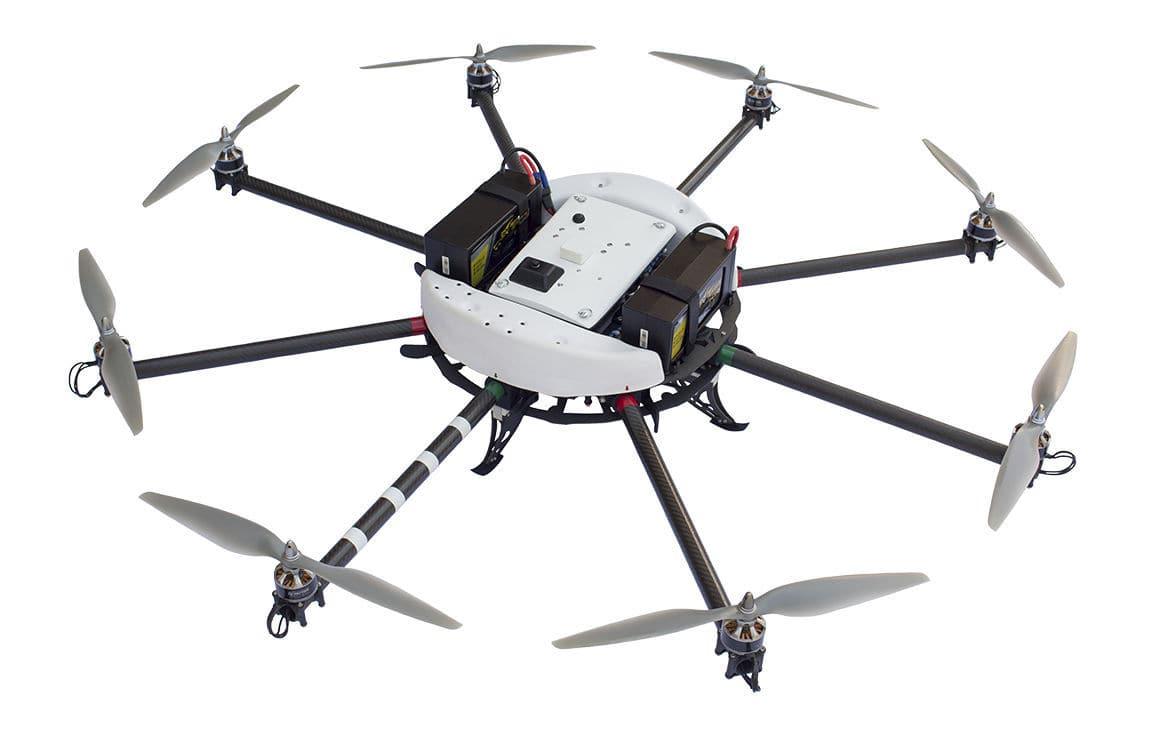
\includegraphics[width=8.0cm]{rotarywinguav.jpg}    
\caption[Octorotor rotary-wing UAV]{Octorotor rotary-wing UAV\protect\footnotemark} 
\label{fig:rotarywing}
\end{center}
\end{figure}
\footnotetext{Rotary-wing UAV image taken from \url{https://goo.gl/hJeFtN}}
\\The main advantage of the rotary-wing UAVs is that they do not need to be constantly moving forward in order to have enough lift that sustains the aircraft in flight, as their propellers rotation generates the lift force by itself. This make the UAV capable of sustaining itself in a desired position.
\\\\
Rotary-wing UAVs do not have control surfaces that change the direction of the air flow in order to control its six $DoF$. Instead, it uses the unbalance of thrust exerted by its motors and propellers to control the rotations of the rigid body and indirectly control its horizontal translational movement. As the motors thrust is always pushing the airframe vertically, the vertical translational movement is independently controlled by the total thrust exerted by all the UAVs motors.
\begin{figure}[H]
\begin{center}
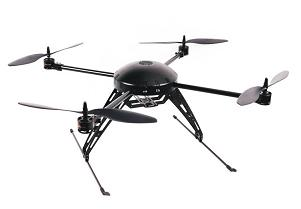
\includegraphics[width=8.0cm]{quadrotor.jpg}    
\caption[Quadrotor aircraft X650]{Quadrotor aircraft X650 \protect\footnotemark} 
\label{fig:quadrotarywing}
\end{center}
\end{figure}
\footnotetext{Quadrotor XAircraft X650 image taken from \url{https://goo.gl/ug5FJs}}
Due to the simplicity in its construction, the most common small-size rotary-wing UAV type developed by manufacturers and hobbyists, is the quadrotor. The quadrotors, also known as quadcopters, are typically based on a light airframe built with fiberglass or carbon fiber, and four motors that serve as actuation devices, as shown in Fig. \ref{fig:quadrotarywing}. This aircrafts  can be built in a relatively simple and inexpensive manner, besides being easy to control and model, when being compared with other multirotors. This is the reason why a quadrotor was established as the experimental platform in this project.
\\\\
\section{Literature Review}
In this section, the literature review regarding the research done about control strategies and state estimation algorithms for quadrotors, is shown. Also, the main quadrotor flight modes, widely used in commercial flight controllers are detailed. Finally, the smartphones capabilities within control systems are studied.

\subsection{Control Strategies and State Estimation in Quadrotors}
Since UAVs represent a challenge for the modelling and design of controllers, from basic to advanced, these aircrafts are widely used in teaching and research of control systems. For instance, \cite{Argentim2013} implemented a PID controller (with two tuning methods) and a Linear-Quadratic regulator (LQR) for altitude control in a quadrotor, comparing them and establishing the advantages of using a PID controller tuned using the LQR equations. Moreover, \cite{Silva2016} exposes the develop of a low cost quadrotor attitude controler based on a PID control strategy with saturation constraints, achieving the quadrotor attitude stabilization with set-points of less than $0.23\ rad$. Another comparison between PID and LQR control strategies is done in \cite{Liu2016}. In this case, both controllers are used for trajectory tracking in a Qball-X4 quadcopter, getting smoother results with the LQR implementation.
\\\\
In \cite{Reyes-Valeria2013}, a quaternion-based LQR gain scheduling controller is designed and simulated, successfully achieving six $DoF$ control of the quadrotor. A position and heading regulation system using a LQR is also presented in \cite{Dong2015}. Here, the implementation of the designed controller is carried out, in which the altitude regulation with oscillations of $0.1\ m$ is observed. On the other hand, \cite{Fan2017} designed a feed-forwarding LQR, which achieve to control quadrotor attitude with errors of less than $0.08\ rad$.
\\\\
As a parallel work to this thesis, in \cite{Munoz2017} the altitude and attitude control strategies for a smartphone-based quadrotor were designed and implemented. Here, cascade PID controllers for translational and rotational position and velocities were tested. The $x$ and $y$ position dynamics were neglected in this project.
\\\\
A trajectory tracking controller based on a LQR and an Extended Kalman Filter (EKF) is shown in \cite{Zhang2016}. This approach uses the non-linear quadrotor dynamics model to estimate the quadrotor states and calculte the control signals based on the estimations.
\\\\
Another quadrotor control strategy found in literature is the Model Predictive Control (MPC). In \cite{Configuration2017}, a MPC controller for trajectory tracking is compared to a PID controller, getting an improvement in setting time and overshoot. \cite{Castillo201603a} proposed a non-linear quaternion based control law complemented with an active disturbance rejection strategy that attempts to control the attitude of a quadrotor.
\\\\
In \cite{Ameho2013}, a Linear Parameter-Varying (LPV) control strategy is developed. Here, an adaptive control is implemented in order to control independently a family of multi-sized quadrotors using the same controller approach. On the other hand, \cite{Gao2015} proposes a fuzzy adaptive sliding mode
controller that aims to overcome actuators fault within the quadrotor attitude control system. Another adaptive control strategy was developed in \cite{Wang2017a}, \cite{Emran2015} and \cite{Wang2017}, where parameters uncertainties were taken into account in order to control the variable payload quadrotors.
\\\\
Finally, in \cite{Prayitno2016} and \cite{Ortiz2016}, the authors designed $H_{\infty}$ controllers for reference tracking in quadrotors, evidencing the implementation advantages of this controller in terms of robustness.
\\\\
Regarding about state estimation in quadrotors, after a literary review, it was found that the Kalman filter (KF) is a widely used estimation algorithm in all its different variants. For instance, in \cite{Munoz2017}, a KF for altitude estimation based on the model of a moving particle was developed. A two stage KF for both quadrotor state and parameter estimation is presented in \cite{Moghadam2015}. This KF is designed in order to detect and identify fails in the quadrotor actuators. As the quadrotor dynamic model is strictly non-linear, the EKF is a popular variation of the KF used in multiple ongoing research, such as \cite{Goodarzi2016}, \cite{Oh2015}, and \cite{Sebesta2014}. Other variation of the KF is the Unscented Kalman Filter (UKF) which uses a deterministic sampling approach in order to estimate the state of a non-linear model. In \cite{Goslinski2013}, an UKF is used to estimate the orientation of a quadrotor on a test bench, comparing its estimations with the measurements of an incremental encoder and the estimations of a standard KF. The results of this comparison show that the UKF estimations are more similar to the measured orientation, than the estimates of KF.
\\\\
In \cite{AlYounes2015}, a model-free technique implemented within a Thau observer is presented. This state estimator aims to compensate uncertainties and unmodeled dynamics. Also, other projects have used on board cameras, for the acquisition of extra data that improve the state estimation, as seen in \cite{Xie2016}, \cite{Yu2017} and \cite{Liu2017}, demonstrating that the use of vision-based odometry improves the quadrotor state estimation despite depending on inaccurate sensors.

\subsection{Quadrotor Flight Modes}
%\url{http://ardupilot.org/copter/docs/flight-modes.html}
In quadrotors, the on board flight controllers keep some of the quadrotors $DoF$ in a desired value autonomously in order to allow pilots to perform tasks during a flight. This controllers have different modes that can control from three to six $DoF$ depending on the will of the pilot. Flight modes commonly found in commercial flight controllers may be as basic to only control its attitude or as complex to let the quadrotor follow a complex trajectory with multiple waypoints \cite{Ardupilot2016}.
\\\\
The main flight modes, widely used in commercial flight controllers, are described bellow according to the number of controlled $DoF$, in ascending order.

\begin{itemize}
\item \textbf{Stabilize Mode}\\\\
This mode allows the pilot to fly the quadrotor manually while the flight controller self-levels the quadrotor attitude and regulate its current heading. Thus, the stabilize mode attempts to control three $DoF$ of the quadrotor.\\\\
The attitude references can be set or changed by the pilot using the remote control, but their default value is $0\ rad$. On the other hand, the quadrotor heading is simply set to be regulated in its current state, enabling its rate using the remote control.
\\\\
Since the stabilize mode do not take into account the control of the quadrotor position, the pilot needs to regularly change the attitude references manually to keep the quadrotor in a desired position, as it is affected by wind disturbances. Also, the pilot needs to regularly adjust the quadrotor thrust, so a desired altitude is maintained.

\item \textbf{Altitude Hold Mode}\\\\
The altitude hold mode adds automatic altitude control to the stabilize mode. This way, the quadrotor thrust is set by the flight controller in order to keep the quadrotor in a desired altitude, attaining four controlled $DoF$.
\\\\
In this mode, the pilot can remotely control the rate of altitude change (with a default value of $0\ m/s$), as well as the attitude references.

\item \textbf{GNSS-Dependent Flight Modes}\\\\
The Global Navigation Satellite System (GNSS)-Dependent flight modes, are those that automatically attempt to regulate the six $DoF$ of the quadrotor in order to maintain a desired position, heading and altitude during a flight. The main GNSS-Dependent Flight Modes are: Loiter mode, Auto Mode, and Return-To-Launch (RTL) Mode.
\\\\
In Loiter mode, the quadrotor attitude is self-leveled, while the position and altitude reference can be modified by the pilot using the remote controller. The position and altitude references are initialized using the current quadrotor position and altitude when this mode is set. 
\\\\
The Auto mode attempts to make a quadrotor follow automatically a pre-programmed path connecting multiple position and heading waypoints. This mode uses the same controller as the Loiter mode, but its references are set automatically following a list of waypoints. 
\\\\
During a flight mission, the home location is set as the position and altitude where the quadrotor took off. The RTL mode is used in case of emergency or when a the last waypoint is reached within a flight mission. This mode is equivalent to the Auto mode, but only has two waypoints. The first waypoint consists in the position of the home location with a previously set security altitude ($RTL$ altitude) greater than the take-off altitude. When this waypoint is reached, the home location is set as the following waypoint so the quadrotor starts its landing, while keeping the position controlled.
\end{itemize}



\subsection{Smartphones in Control Systems}
Current smartphone processors are able to perform complex calculations such as those required in the implementation of real time control strategies. Multiple research projects have been carried out using smartphones as tools for development of control systems in robotics.
\\\\
A survey about the trend of using smartphones as main processing component in robotics for research and education was carried out in \cite{Oros2013a}.
In \cite{DeABarbosa2015}, it is proposed a low cost differential robot controlled using a smartphone as processing and sensing device, taking advantage of the ROS framework for Android. \cite{Gunawan2014} expose the development of an adaptive cruise control algorithm for an object-following robot controlled by a smartphone on board. Also, an autonomous smartphone-based robot platform for football competitions, exposed in Fig. \ref{fig:soccer}, was designed and shown in \cite{Tetzlaff2013}.
\begin{figure}[H]
\begin{center}
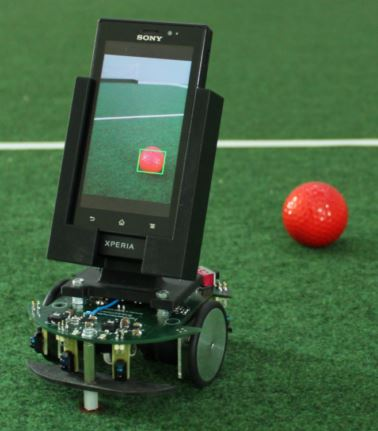
\includegraphics[width=6.5cm]{soccerrobot.jpg}    
\caption[Smartphone-based ball tracking robot]{Smartphone-based ball tracking robot \protect\footnotemark} 
\label{fig:soccer}
\end{center}
\end{figure}
\footnotetext{Smartphone-based ball tracking robot image taken from \cite{Tetzlaff2013}}
There are many ongoing research related to the possibility of using smartphones to implement control strategies \cite{Drumea2013a}, as configuration and monitoring interfaces in control systems \cite{Lin2014a,Truong2012a, Lu2017}, and as a tool in both education and design of control strategies \cite{Aristizabal2014a,WuWu2013a}. Following this trend, in the Universidad del Valle, it was developed a smartphone-based platform for monitoring, control and communication in portable laboratories, where a controller for a pendulum, based in the Lego Mindstorms EV3 platform, was implemented \cite {GarciaTellez2015}.

\subsection{Smartphone-based Quadrotors}
Multiple attempts to unite the technologies of quadrotors and smartphones have been made. Some of this attempts are described below.
\\\\
In \cite{Isuru2017}, the possibility of using old discarded smartphones as sensors and processor in a quadrotor was studied. In \cite{Pearce2014a}, a smartphone was used as mission planner for a quadrotor using a commercial flight controller on board. \cite{ALEMARK2014a} implemented a flight control system in a smartphone, using its sensors and computational power to stabilize the quadrotor attitude and control its altitude. Also, in the University of Pennsylvania \cite{Loianno2015}, a Google Tango smartphone was used as a quadrotor flight controller, including an image-based positioning system based on RGB-D images captures. The state estimation algorithms, control and planning were firstly implemented in a ODROID-XU board with additional sensors, but then, in \cite{Loianno2015a}, this algorithms were ported to the processor of the updated smartphone used in the project. The quadrotor developed in this project is shown in Fig. \ref{fig:penn}.
\begin{figure}[h]
\begin{center}
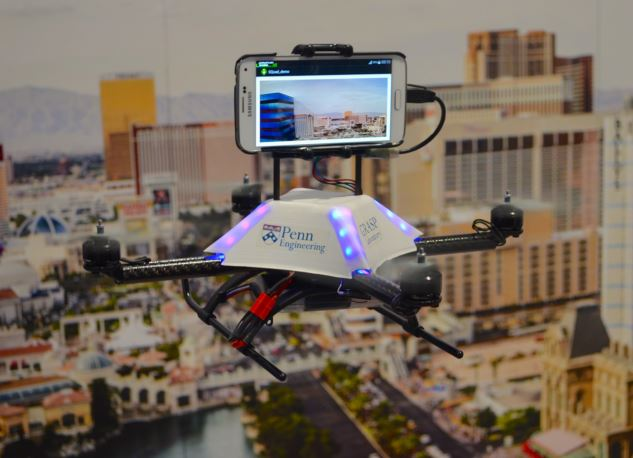
\includegraphics[width=8.0cm]{penn.jpg}    
\caption[UPenn's smartphone-based quadrotor]{UPenn's smartphone-based quadrotor \protect\footnotemark} 
\label{fig:penn}
\end{center}
\end{figure}
\footnotetext{UPenn smartphone-based quadrotor image taken from \cite{Loianno2015a}}
\\
In \cite{Alsharif2016}, a PID controller aimed to be executed in a smartphone on board a quadrotor, which is also responsible for estimating the rotational dynamics of the quadrotor using the measurements made by the smartphone, was implemented. Following this project, \cite{Alsharif2017} exposes in detail the development of a model-free PID controller for a smartphone-based quadrotor, including the processing of delayed feedback in the controller. After that, in \cite{Alsharif2017a}, a LQR controller with integral feedback (LQI) was implemented and compared with the model-free PID controller set before. 
Finally, \cite{Aldrovandi2015} developed a non-linear complementary filter for position and attitude estimation in a smartphone-based quadrotor.

\subsubsection{Smartphone-based Quadrotor Limitations}
The idea of using a smartphone as flight controller in an UAV opens the possibility of a quick and inexpensive development task \cite{Aldrovandi2015}. A smartphone offers other advantages compared with off-the-shelf flight controllers, for instance its powerful quad, hexa or octa-core processors and communications interfaces. However, smartphones and the Android operating system have some limitations that set challenges when implementing a control system in it.\\\\
Android is not a real-time operating system and therefore, can not assure execution of algorithms, like estimation and control, with a constant sample time. Furthermore, the sensors embedded in commercial smartphones are made for applications that do not have high requirements of accuracy nor precision, and therefore may not be appropriate for sensing quadrotor dynamics. Nonetheless, as explained by \cite{Bryant2015}, due to its computing capabilities, smartphones can overcome this limitations while using a temporized thread to execute the control system algorithms and implementing a sensor fusion technique to improve the states estimation reliability. This thread must be executed with a lower sample time compared to the one of the sensors embedded in the smartphone. This will ensure that the execution is not delayed by the sensors acquisition process.

\section{Research Problem}
The existing research challenges include how to develop and implement efficient control algorithms for smartphones using the Android operating system, and assess, adapt and develop the appropriate communication, sensing and performance technologies with smartphones in the execution of missions using quadrotors.
\\\\
Then, the question to be answered is: how to develop control strategies in a smartphone in order to control the flight dynamics of a quadrotor so it can develop flight missions while the instrumentation and computing capacity of the smartphone is used?

\section{Objectives}
In order to find a solution for the research problem, the following general and specific objectives are proposed:
\subsubsection{General Objective}
Design and implement algorithms for control and estimation of flight dynamics executed in a smartphone for the quadrotor of the Industrial Control Research Group.
\subsubsection{Specific Objectives}
\begin{itemize}
\item Conduct a study and analysis of the state of the art related to the control and estimation of states of quadrotors.
\item Integrate the existing quadrotor with a smartphone that contains the appropriate sensors for the control and estimation of states.
\item Obtain a dynamic model of the quadrotor.
\item Design and implement the algorithms for control and estimation of states for the quadrotor.
\item Integrate the experimentation platform with the control and estimation algorithms in the smartphone.
\item Evaluate the performance of the control strategies.%????
\end{itemize}

\section{Contribution of this Work}
With respect to the works analyzed in the literary review, the development of this thesis led to make some contributions that are worth mentioning:
\begin{itemize}
\item The two main configuration of quadrotor geometries are detailed. Here, is shown the input settings and the maximum available torque for both configurations. This facilitates the analysis of the advantages of building one or the other.
\item The dynamic model of the quadrotor is derived from both the Newton-Euler and Euler-Lagrange approaches. Additionally, the Jacobian linearization procedure and the practical requirement of thrust compensation are explained. 
\item The simple experimental procedure for the identification of the quadrotor parameters is detailed.
\item Dynamical controllers, such as the $H_\infty$ controllers designed for multiple flight modes, are implemented in Android. Additionally, the developed application executes a Kalman filter and quadratic linear regulators with integral feedback. This allows to compare the performance of each controller depending on the controlled quadrotor dynamics.
\item A complete unmanned aerial system was designed and implemented. This includes the smartphone-based quadrotor prototype, a cross-platform ground control station, and a WLAN-based communication channel between them.
\end{itemize}


\section{Outline}
This thesis is organized as follows.\\\\
In Chapter \ref{ch:introduction}, the motivation and scope of this project are presented. After that, the definition and classification of UAVs are given. Finally, a short literature review regarding control and estimation in quadrotors, flight modes, and smartphones in control systems, is detailed.
\\\\
The dynamic model of the quadrotor is described in Chapter \ref{ch:model}. Here, the non-linear and linearized quadrotor model are obtained taking into account the main quadrotor geometry configurations and their input setting. 
\\\\
Chapter \ref{ch:prototype} focuses on the smartphone-based quadrotor prototype description, detailing all its components and their interactions, as well as the specific parameters of the prototype.
\\\\
The design of the control and estimation algorithms is presented in Chapter \ref{ch:controlandestimation}. In this chapter, specific controllers for each quadrotor flight mode are designed and simulated.
\\\\
In Chapter \ref{ch:implementation}, the implementation results of the control and estimation algorithms, as well as the description of the Android application and the GCS are detailed.
\\\\
Finally, in Chapter \ref{ch:conclusions}, the thesis conclusions and suggestions for future developments and improvements, are shown.